\mode*

\section{Översikt}

\begin{frame}[fragile]
  \begin{block}{Händelsebaserat}
    \begin{itemize}
      \item Oändlig slinga som läser meddelanden från OS.
      \item OS skickar ett meddelande per händelse.
    \end{itemize}
  \end{block}
\end{frame}


\section{tkinter-biblioteket}

\begin{frame}[fragile]
  helloworld.py \hrulefill
  \inputminted[linenos]{python}{examples/helloworld.py}
\end{frame}

\begin{frame}
  \centering
  \begin{figure}
    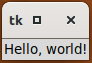
\includegraphics{figs/helloworld.png}
    \caption{Fönstret som genereras av helloworld.py.}
  \end{figure}
\end{frame}

\subsection{Inmatning och utmatning}

\begin{frame}
  \begin{figure}
    \begin{subfigure}{\columnwidth}
      \centering
      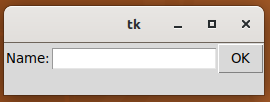
\includegraphics[height=0.3\textheight]{figs/hello_user.png}
      \caption{Ett program med textfält för inmatning.}
    \end{subfigure}
    \begin{subfigure}{\columnwidth}
      \centering
      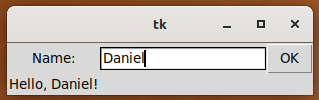
\includegraphics[height=0.3\textheight]{figs/hello_user_daniel.png}
      \caption{Samma program med inmatning och utmatning.}
    \end{subfigure}
    \caption{Skärmdumpar av ett grafiskt gränssnitt med in- och utmatning.}
  \end{figure}
\end{frame}

\begin{frame}[fragile]
  hello\textunderscore user\textunderscore bad.py \hrulefill
  \inputminted[linenos,firstline=7,lastline=19]{python}{examples/hello_user_bad.py}
\end{frame}

\begin{frame}[fragile]
  hello\textunderscore user\textunderscore bad.py \hrulefill
  \inputminted[linenos,firstline=21,lastline=31]{python}{examples/hello_user_bad.py}
\end{frame}

\begin{frame}
  \begin{remark}
    \begin{itemize}
      \item Vi kan använda klasser istället!
    \end{itemize}
  \end{remark}
\end{frame}

\begin{frame}[fragile]
  hello\textunderscore user\textunderscore good.py \hrulefill
  \inputminted[linenos,lastline=12]{python}{examples/hello_user_good.py}
\end{frame}

\begin{frame}[fragile]
  hello\textunderscore user\textunderscore good.py \hrulefill
  \inputminted[autogobble=false,linenos,firstline=18,lastline=25]{python}{examples/hello_user_good.py}
  \dots
  \inputminted[autogobble=false,linenos,firstline=30,lastline=32]{python}{examples/hello_user_good.py}
\end{frame}

\begin{frame}[fragile]
  hello\textunderscore user\textunderscore counter.py \hrulefill
  \inputminted[linenos,firstline=5,lastline=14]{python}{examples/hello_user_counter.py}
  \dots
  \inputminted[autogobble=false,linenos,firstline=32,lastline=34]{python}{examples/hello_user_counter.py}
\end{frame}

\subsection{Enklare med arv}

\begin{frame}[fragile]
  hello\textunderscore user\textunderscore better.py \hrulefill
  \inputminted[linenos,firstline=5,lastline=13]{python}{examples/hello_user_better.py}
  \dots
  \inputminted[linenos,firstline=33,lastline=38]{python}{examples/hello_user_better.py}
\end{frame}

\begin{frame}[fragile]
  hello\textunderscore user\textunderscore even\textunderscore better.py
  \hrulefill
  \inputminted[linenos,firstline=5,lastline=9]{python}{examples/hello_user_even_better.py}
  \dots
  \inputminted[autogobble=false,linenos,firstline=24,lastline=32]{python}{examples/hello_user_even_better.py}
\end{frame}

\subsection{Annan typ av inmatning}

\begin{frame}
  \begin{figure}
    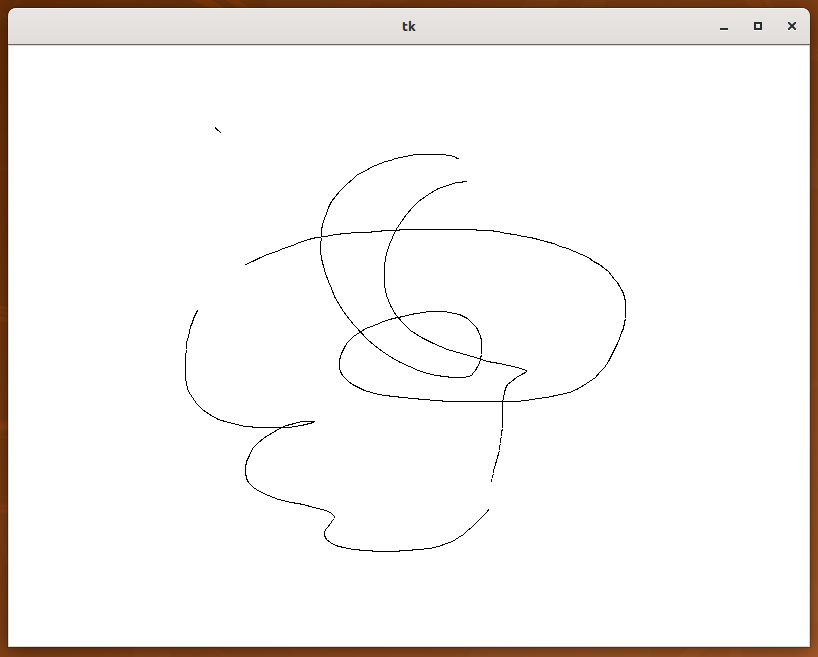
\includegraphics[height=0.5\textheight]{figs/draw.png}
    \caption{Skärmdump av program där man ritar med musen.}
  \end{figure}
\end{frame}

\begin{frame}[fragile]
  draw.py \hrulefill
  \inputminted[linenos,firstline=5,lastline=13]{python}{examples/draw.py}
  \dots
  \inputminted[autogobble=false,linenos,firstline=18,lastline=22]{python}{examples/draw.py}
\end{frame}

\begin{frame}
  \href{http://effbot.org/tkinterbook/tkinter-events-and-bindings.htm}{%
    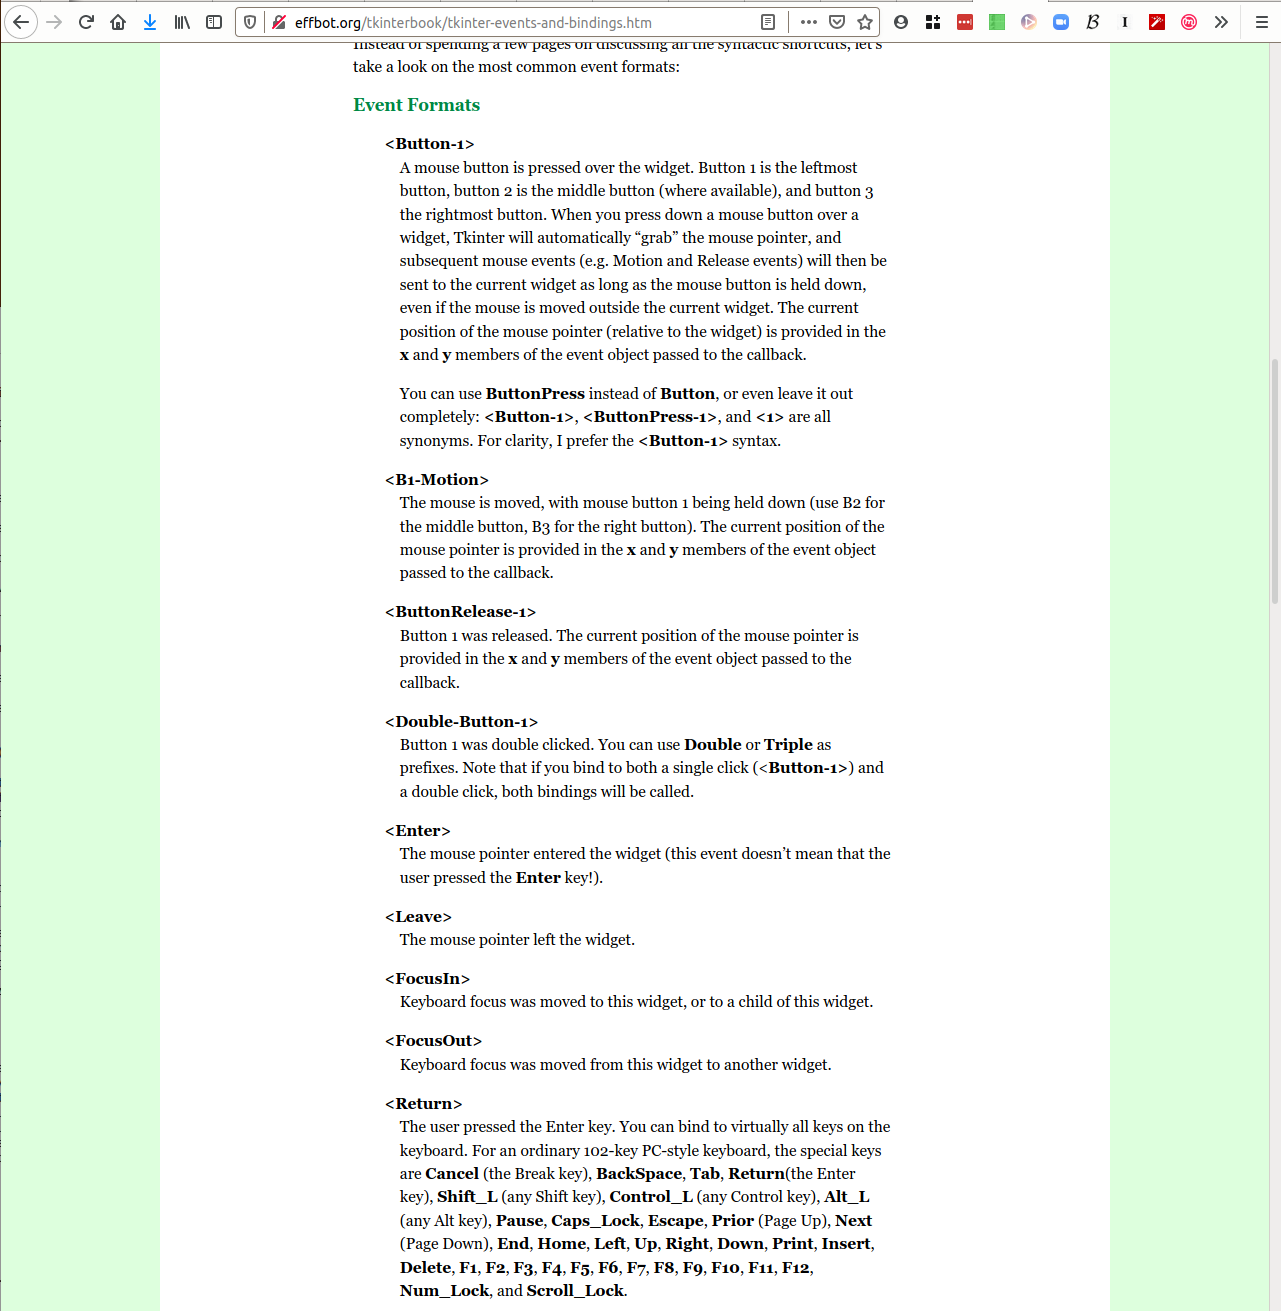
\includegraphics[width=\columnwidth]{figs/docs-events.png}
  }
\end{frame}

\begin{frame}[fragile]
  draw.py \hrulefill
  \inputminted[linenos,firstline=24,lastline=40]{python}{examples/draw.py}
\end{frame}

\begin{frame}
  \href{http://effbot.org/tkinterbook/canvas.htm\#Tkinter.Canvas.create_line-method}{%
    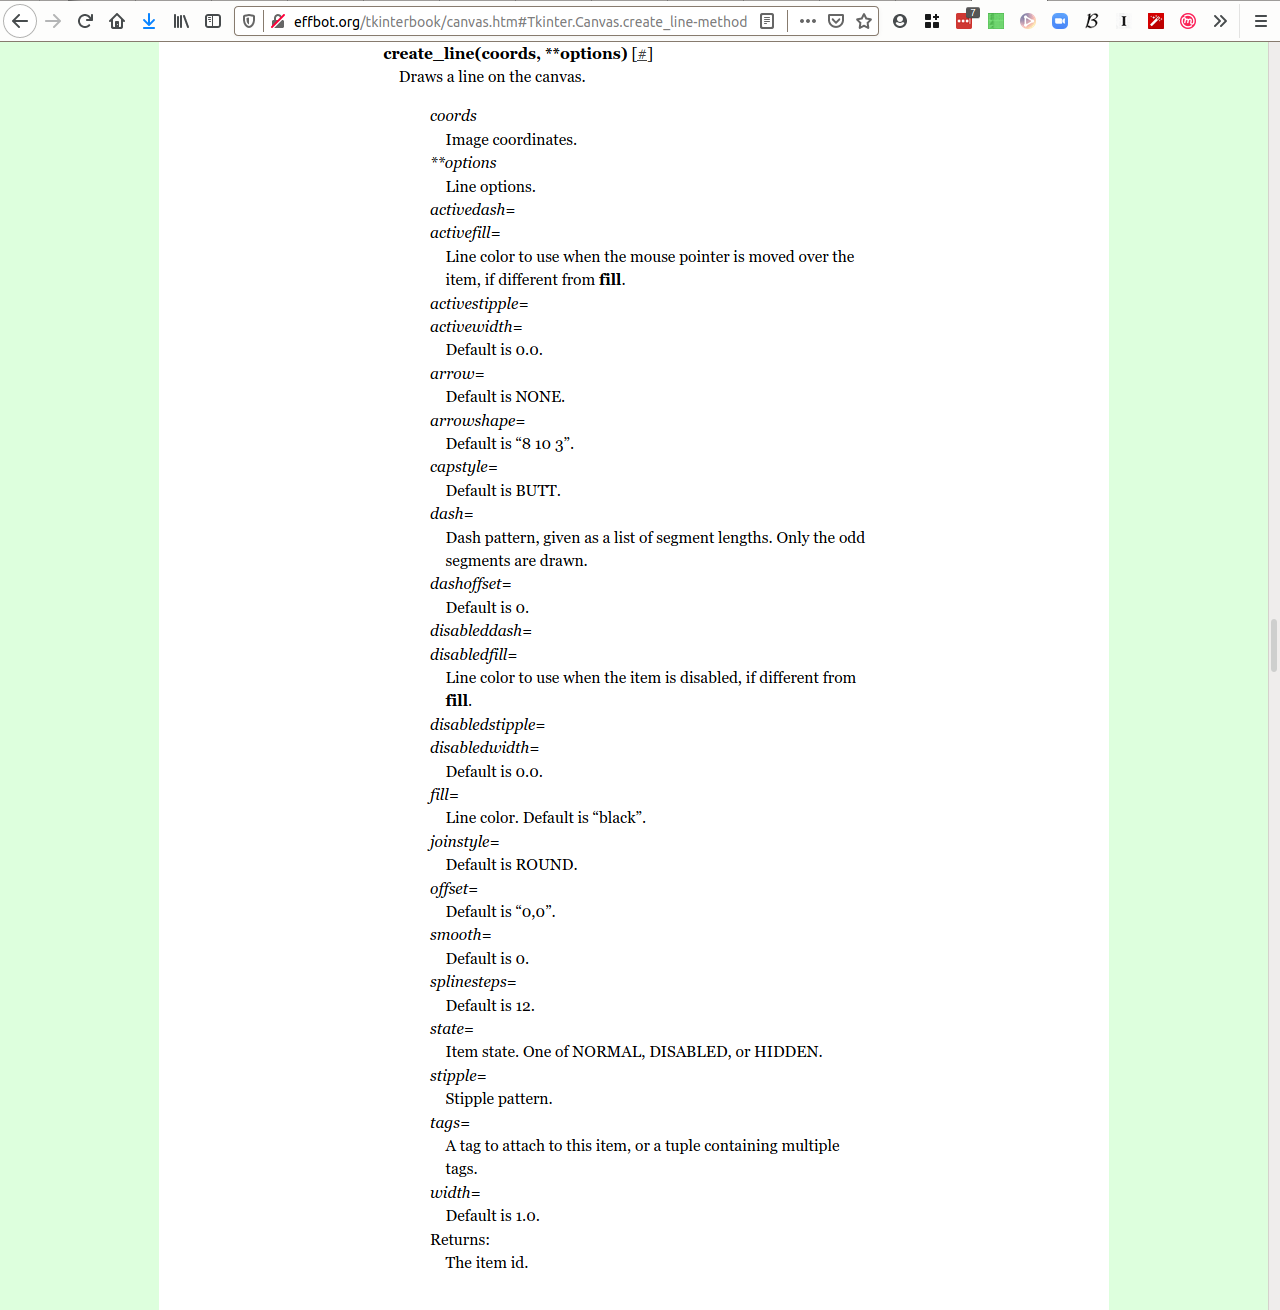
\includegraphics[width=\columnwidth]{figs/docs-create_line.png}
  }
\end{frame}

\begin{frame}
  \begin{question}
    \begin{itemize}
      \item Hur mycket meddelanden/händelser hanterar vi?
    \end{itemize}
  \end{question}

  \pause

  \begin{solution}
    \begin{itemize}
      \item Vi kan testa med draw\textunderscore debug.py.
    \end{itemize}
  \end{solution}
\end{frame}

\begin{frame}
  \begin{exercise}
    \begin{itemize}
      \item Hur kan vi lägga till knappar för att byta färg?
    \end{itemize}
  \end{exercise}
\end{frame}

\begin{frame}[fragile]
  draw\textunderscore colors.py \hrulefill
  \inputminted[linenos,firstline=5,lastline=7]{python}{examples/draw_colors.py}
  \dots
  \inputminted[autogobble=false,linenos,firstline=27,lastline=34]{python}{examples/draw_colors.py}
\end{frame}

\begin{frame}[fragile]
  draw\textunderscore colors.py \hrulefill
  \inputminted[autogobble=false,linenos,firstline=40,lastline=40]{python}{examples/draw_colors.py}
  \dots
  \inputminted[autogobble=false,linenos,firstline=49,lastline=52]{python}{examples/draw_colors.py}
  \dots
  \inputminted[autogobble=false,linenos,firstline=58,lastline=60]{python}{examples/draw_colors.py}
\end{frame}
